\begin{table}
\begin{adjustbox}{max totalheight=\textheight}
    \begin{tabular}{|l|ll|llllll|}
    \hline
    ~                  & DDD   & ~      & LDD  & ~    & ~    & ~    & ~     & ~     \\ \hline
    ~                  & ~     & no-min & ~    & gsa  & rb4w & cw   & rs,rn & rs,ru \\ \hline
    fischer1           & 0.8   & 0.8    & 0.8  & 1.1  & 0.8  & 0.8  & 0.8   & 0.8   \\
    fischer2           & 0.9   & 0.9    & 0.9  & 1.5  & 0.9  & 0.9  & 0.9   & 0.9   \\
    fischer3           & 0.9   & 0.9    & 0.9  & 2.0  & 0.9  & 0.9  & 0.9   & 0.9   \\
    fischer4           & 1.2   & 1.2    & 1.2  & 2.9  & 1.3  & 1.2  & 1.2   & 1.2   \\
    fischer5           & 14.1  & 10.2   & 6.1  & 9.3  & 7.3  & 6.5  & 6.1   & 5.9   \\
    critRegion1        & 0.9   & 0.9    & 0.9  & 1.2  & 0.9  & 0.9  & 0.8   & 0.8   \\
    critRegion2        & 0.9   & 0.9    & 0.9  & 1.5  & 0.9  & 0.9  & 0.9   & 0.9   \\
    critRegion3        & 3.7   & 3.6    & 1.8  & 2.8  & 1.9  & 1.8  & 1.7   & 2.2   \\ \hline
    Critical\_01-25-50 & 0.9   & 0.9    & 0.9  & 1.3  & 0.9  & 0.9  & 0.9   & 0.9   \\
    Critical\_02-25-50 & 0.9   & 1.0    & 1.0  & 1.6  & 1.0  & 1.0  & 0.9   & 1.0   \\
    Critical\_03-25-50 & 13.8  & 13.8   & 7.2  & 9.9  & 9.3  & 7.4  & 6.9   & 11.6  \\ \hline
    CSMACD\_01         & 0.8   & 0.8    & 0.8  & 1.0  & 0.8  & 0.8  & 0.8   & 0.8   \\
    CSMACD\_02         & 1.0   & 1.0    & 1.0  & 1.3  & 1.0  & 1.0  & 1.0   & 1.0   \\
    CSMACD\_03         & 1.0   & 1.0    & 1.0  & 1.5  & 1.0  & 1.0  & 1.0   & 1.0   \\
    CSMACD\_04         & 1.2   & 1.2    & 1.2  & 1.7  & 1.2  & 1.1  & 1.2   & 1.1   \\
    CSMACD\_05         & 1.9   & 1.4    & 1.5  & 2.1  & 1.5  & 1.5  & 1.4   & 1.4   \\
    CSMACD\_06         & 5.0   & 2.0    & 2.6  & 3.2  & 2.6  & 2.6  & 2.4   & 2.4   \\
    CSMACD\_07         & 19.7  & 3.7    & 7.2  & 7.6  & 7.4  & 7.4  & 6.5   & 6.4   \\
    CSMACD\_08         & 237.0 & 10.4   & 26.7 & 25.5 & 28.0 & 28.0 & 23.5  & 22.8  \\ \hline
    viking1            & 0.8   & 0.8    & 0.8  & 1.1  & 0.8  & 0.8  & 0.8   & 0.8   \\
    viking2            & 0.9   & 0.9    & 0.9  & 1.3  & 0.9  & 0.9  & 0.9   & 0.9   \\
    viking3            & 0.9   & 0.9    & 0.9  & 1.5  & 0.9  & 0.9  & 0.9   & 0.9   \\
    viking4            & 1.0   & 1.0    & 1.0  & 1.7  & 1.0  & 1.0  & 1.0   & 1.0   \\
    viking5            & 1.1   & 1.1    & 1.1  & 2.0  & 1.1  & 1.1  & 1.1   & 1.1   \\
    viking6            & 1.7   & 1.7    & 2.0  & 2.9  & 2.0  & 2.0  & 1.8   & 1.7   \\
    viking7            & 2.2   & 2.2    & 2.5  & 3.6  & 2.5  & 2.5  & 2.2   & 2.1   \\
    viking8            & 4.7   & 4.7    & 5.8  & 6.4  & 5.9  & 5.9  & 4.9   & 4.4   \\
    viking9            & 12.1  & 12.2   & 16.2 & 14.9 & 16.4 & 16.3 & 13.1  & 11.5  \\
    viking10           & 33.9  & 34.0   & 46.9 & 38.9 & 47.2 & 47.3 & 37.1  & 31.5  \\ \hline
    Lynch1-16          & 0.8   & 0.8    & 0.8  & 1.4  & 0.8  & 0.8  & 0.8   & 0.8   \\
    Lynch2-16          & 0.9   & 0.9    & 0.9  & 2.2  & 0.9  & 0.9  & 0.9   & 0.9   \\
    Lynch3-16          & 1.3   & 1.3    & 1.2  & 3.3  & 1.3  & 1.2  & 1.2   & 1.2   \\
    Lynch4-16          & 8.8   & 8.6    & 8.4  & 11.3 & 10.0 & 8.6  & 8.2   & 8.0   \\ \hline
    bocdp              & 1.6   & 1.6    & 1.6  & 14.6 & 1.6  & 1.6  & 1.6   & 1.6   \\
    bocdpFIXED         & 1.6   & 1.6    & 1.6  & 13.5 & 1.6  & 1.6  & 1.6   & 1.5   \\
    bando              & 1.6   & 1.6    & 1.5  & 13.5 & 1.6  & 1.6  & 1.5   & 1.5   \\
    timelock           & 0.7   & 0.7    & 0.7  & 0.9  & 0.7  & 0.7  & 0.7   & 0.7   \\ \hline
    Milner-2Nodes-flat & 0.9   & 0.9    & 0.9  & 1.3  & 0.9  & 0.9  & 0.9   & 0.9   \\
    Milner-3Nodes-flat & 1.0   & 0.9    & 1.0  & 1.6  & 1.0  & 1.0  & 1.0   & 1.0   \\
    Milner-4Nodes-flat & 1.1   & 1.0    & 1.6  & 2.2  & 1.6  & 1.6  & 1.5   & 1.5   \\
    Milner-5Nodes-flat & 1.2   & 1.2    & 2.1  & 2.9  & 2.1  & 2.1  & 2.1   & 2.0   \\
    Milner-6Nodes-flat & 1.5   & 1.4    & 3.0  & 3.8  & 3.0  & 3.0  & 2.8   & 2.7   \\
    Milner-7Nodes-flat & 1.8   & 1.7    & 4.2  & 5.2  & 4.3  & 4.3  & 4.0   & 3.8   \\
    Milner-8Nodes-flat & 2.3   & 2.2    & 6.1  & 7.0  & 6.2  & 6.2  & 5.5   & 5.2   \\ \hline
    hddi\_input\_1     & 0.9   & 0.9    & 0.9  & 1.0  & 0.9  & 0.9  & 0.9   & 0.9   \\
    hddi\_input\_2     & 1.0   & 0.9    & 0.9  & 1.2  & 0.9  & 0.9  & 0.9   & 0.9   \\
    hddi\_input\_3     & 179.4 & 1.0    & 1.1  & 1.4  & 1.1  & 1.1  & 1.1   & 1.1   \\
    ANIMO\_small       & 1.1   & 1.1    & 1.1  & 1.8  & 1.1  & 1.1  & 1.1   & 1.1   \\ \hline
    \end{tabular}
\end{adjustbox}
\end{table}

\begin{table}
\begin{adjustbox}{max totalheight=\textheight}
    \begin{tabular}{|l|ll|llllll|}
    \hline
    ~                  & DDD    & ~        & LDD    & ~      & ~      & ~      & ~      & ~      \\ \hline
    ~                  & ~      & no-minus & ~      & gsa    & rb4w   & cw     & rs,rn  & rs,ru  \\ \hline
    fischer1           & 14     & 14       & 14     & 13     & 14     & 13     & 14     & 14     \\
    fischer2           & 66     & 66       & 66     & 68     & 63     & 66     & 66     & 66     \\
    fischer3           & 509    & 288      & 409    & 505    & 433    & 532    & 409    & 409    \\
    fischer4           & 5025   & 1300     & 2541   & 3905   & 3190   & 4184   & 2541   & 2541   \\
    fischer5           & 49634  & 5535     & 17131  & 30665  & 26004  & 32446  & 17131  & 17131  \\ \hline
    critRegion1        & 24     & 24       & 24     & 24     & 20     & 26     & 24     & 24     \\
    critRegion2        & 251    & 190      & 243    & 358    & 296    & 242    & 243    & 243    \\
    critRegion3        & 4643   & 3825     & 3743   & 5789   & 5506   & 4627   & 3743   & 3743   \\ \hline
    Critical\_01-25-50 & 25     & 25       & 25     & 24     & 23     & 29     & 25     & 25     \\
    Critical\_02-25-50 & 313    & 262      & 316    & 500    & 427    & 370    & 316    & 316    \\
    Critical\_03-25-50 & 12322  & 11183    & 17505  & 29297  & 28443  & 20293  & 17505  & 17505  \\ \hline
    CSMACD\_01         & 17     & 17       & 17     & 17     & 17     & 17     & 17     & 17     \\
    CSMACD\_02         & 112    & 108      & 99     & 101    & 101    & 101    & 99     & 99     \\
    CSMACD\_03         & 686    & 458      & 500    & 553    & 551    & 551    & 500    & 500    \\
    CSMACD\_04         & 3305   & 1356     & 2205   & 2528   & 2520   & 2520   & 2205   & 2205   \\
    CSMACD\_05         & 13867  & 3478     & 8634   & 10154  & 10127  & 10127  & 8634   & 8634   \\
    CSMACD\_06         & 51633  & 7925     & 30862  & 37022  & 36938  & 36938  & 30862  & 30862  \\
    CSMACD\_07         & 176965 & 17069    & 102821 & 125264 & 125019 & 125019 & 102821 & 102821 \\
    CSMACD\_08         & 569760 & 36098    & 324047 & 329844 & 398899 & 398899 & 324047 & 324047 \\ \hline
    viking1            & 12     & 15       & 15     & 15     & 24     & 24     & 15     & 15     \\
    viking2            & 37     & 37       & 37     & 37     & 66     & 66     & 37     & 37     \\
    viking3            & 86     & 86       & 86     & 91     & 176    & 176    & 86     & 86     \\
    viking4            & 105    & 105      & 105    & 111    & 196    & 196    & 105    & 105    \\
    viking5            & 124    & 124      & 124    & 131    & 216    & 216    & 124    & 124    \\
    viking6            & 233    & 233      & 233    & 240    & 504    & 504    & 233    & 233    \\
    viking7            & 190    & 190      & 190    & 199    & 342    & 342    & 190    & 190    \\
    viking8            & 224    & 224      & 224    & 235    & 415    & 415    & 224    & 224    \\
    viking9            & 263    & 263      & 263    & 276    & 495    & 495    & 263    & 263    \\
    viking10           & 304    & 304      & 304    & 317    & 581    & 581    & 304    & 304    \\ \hline
    Lynch1-16          & 24     & 24       & 24     & 22     & 27     & 21     & 24     & 24     \\
    Lynch2-16          & 162    & 162      & 173    & 185    & 217    & 187    & 173    & 173    \\
    Lynch3-16          & 1175   & 922      & 1277   & 1757   & 2600   & 1649   & 1277   & 1277   \\
    Lynch4-16          & 14280  & 8246     & 11113  & 22033  & 32144  & 17146  & 11113  & 11113  \\ \hline
    bocdp              & 541    & 541      & 572    & 329    & 435    & 517    & 572    & 572    \\
    bocdpFIXED         & 542    & 542      & 572    & 428    & 448    & 514    & 572    & 572    \\
    bando              & 542    & 542      & 572    & 428    & 448    & 514    & 572    & 572    \\
    timelock           & 4      & 4        & 4      & 4      & 4      & 4      & 4      & 4      \\ \hline
    Milner-2Nodes-flat & 442    & 245      & 338    & 327    & 394    & 338    & 338    & 338    \\
    Milner-3Nodes-flat & 2709   & 918      & 1602   & 1571   & 1702   & 1602   & 1602   & 1602   \\
    Milner-4Nodes-flat & 4999   & 2968     & 4834   & 4789   & 4997   & 4834   & 4834   & 4834   \\
    Milner-5Nodes-flat & 9106   & 5293     & 8653   & 8596   & 8946   & 8653   & 8653   & 8653   \\
    Milner-6Nodes-flat & 17008  & 7755     & 14100  & 14018  & 14551  & 14100  & 14100  & 14100  \\
    Milner-7Nodes-flat & 25493  & 12188    & 21455  & 21343  & 22098  & 21455  & 21455  & 21455  \\
    Milner-8Nodes-flat & 39887  & 16324    & 31008  & 30884  & 31874  & 31008  & 31008  & 31008  \\ \hline
    hddi\_input\_1     & 221    & 119      & 130    & 134    & 134    & 134    & 130    & 130    \\
    hddi\_input\_2     & 2735   & 693      & 1021   & 1025   & 1090   & 1023   & 1021   & 1021   \\
    hddi\_input\_3     & 20485  & 2013     & 3675   & 3675   & 3971   & 3675   & 3675   & 3675   \\ \hline
    ANIMO\_small       & 235    & 235      & 197    & 191    & 405    & 185    & 197    & 197    \\ \hline
    \end{tabular}
\end{adjustbox}
\end{table}

There is a difference between the number of nodes for the normal BFS and the BFS without minus. This is possible because we do not use a canonical form of DDDs. Most results show a higher number of nodes for the runs with the minus. In figure \ref{fig:fragmentation} we show an example of how this can happen. We assume all zones in the figures belong to the same set of locations. In figure \ref{fig:vis_zone} we have the zone that is already visited. Now a new state with the zone in figure \ref{fig:cur_zone} is discovered. If the minus is not used, successors of this state are directly generated from the set of locations and this zone. If the minus is used the first zone will first be subtracted before successors are generated. The result of the subtraction is shown in figure \ref{fig:after_minus_zone}. This is not a convex zone, so a DDD with multiple paths is needed. From this state also other successors can be generated, possibly needing more nodes to be represented. If the newly generated states are then unioned with the visited set the result can again have more nodes than the version without minus. The less fractionated zones in the current set can also have implications on the time results, as less work in the next-state function is needed. On the other hand the next-state function can also need extra time, as some states would otherwise have completely been removed from the current set, and no work for that states would need to be done. 

In the LDD solution the standard setup with no reordering is for most models faster and uses less nodes than with the reordering algorithms. This is probably due to the densely filled dependency matrices as described in section \ref{subsec:matrices}. If we could make these matrices sparser we expect better results from the reordering algorithms. 

\begin{figure}[h]

\begin{subfigure}[b]{\textwidth}
\centering
\begin{adjustbox}{max totalheight=.3\textheight}
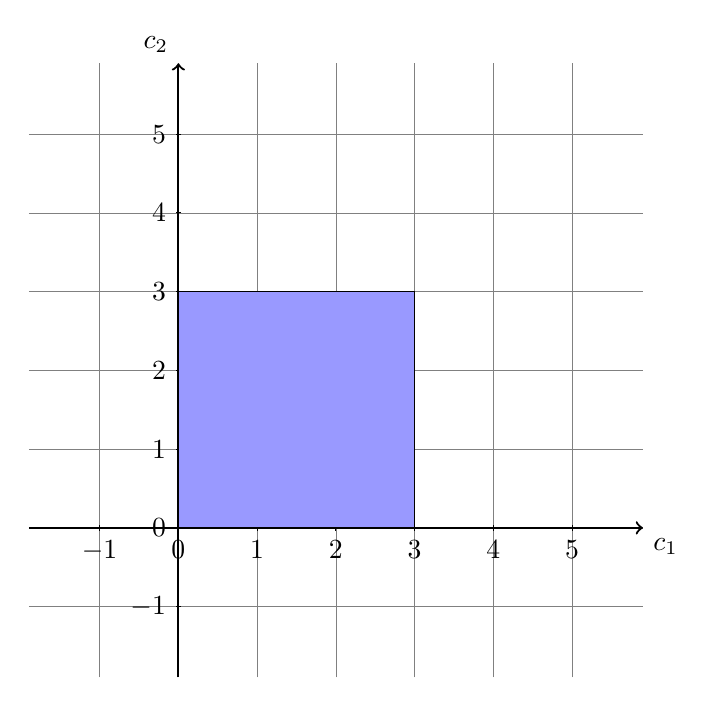
\begin{tikzpicture}

\draw[step=1cm,gray,very thin] (-1.9,-1.9) grid (5.9,5.9);

%\shadedraw[inner color=blue,outer color=red, draw=black] (0,0) rectangle (4,4);

\draw[thick,->] (-1.9,0) -- (5.9,0) node[anchor=north west] {$c_1$};
\draw[thick,->] (0,-1.9) -- (0,5.9) node[anchor=south east] {$c_2$};

\foreach \x in {-1,0,1,2,3,4,5}
    \draw (\x cm,1pt) -- (\x cm,-1pt) node[anchor=north] {$\x$};
\foreach \y in {-1,0,1,2,3,4,5}
    \draw (1pt,\y cm) -- (-1pt,\y cm) node[anchor=east] {$\y$};
    
\filldraw[fill=blue!40!white, draw=black] (0,0) rectangle (3,3);

\end{tikzpicture}
\end{adjustbox}
\caption{Visited Zone}
\label{fig:vis_zone}
\end{subfigure}





\begin{subfigure}[b]{\textwidth}
\centering
\begin{adjustbox}{max totalheight=.3\textheight}
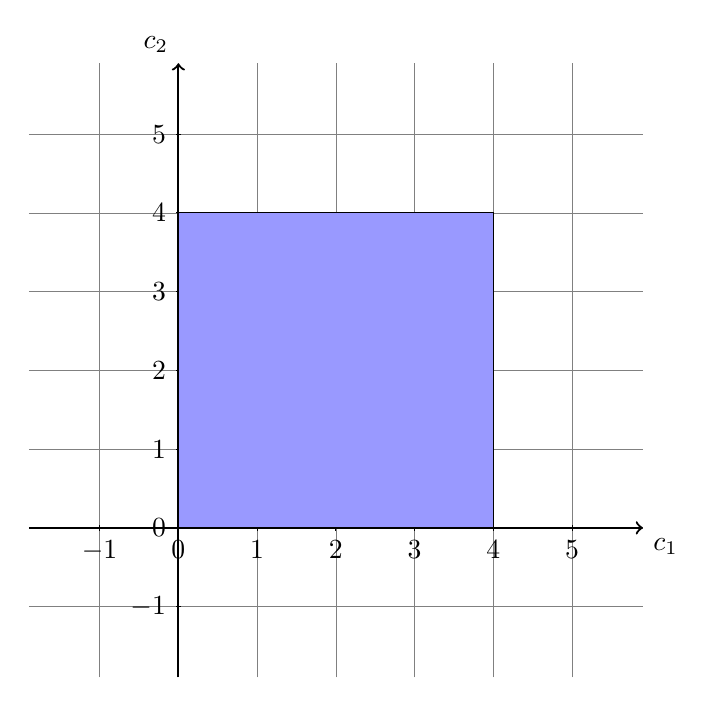
\begin{tikzpicture}
\draw[step=1cm,gray,very thin] (-1.9,-1.9) grid (5.9,5.9);

%\shadedraw[inner color=blue,outer color=red, draw=black] (0,0) rectangle (4,4);

\draw[thick,->] (-1.9,0) -- (5.9,0) node[anchor=north west] {$c_1$};
\draw[thick,->] (0,-1.9) -- (0,5.9) node[anchor=south east] {$c_2$};

\foreach \x in {-1,0,1,2,3,4,5}
    \draw (\x cm,1pt) -- (\x cm,-1pt) node[anchor=north] {$\x$};
\foreach \y in {-1,0,1,2,3,4,5}
    \draw (1pt,\y cm) -- (-1pt,\y cm) node[anchor=east] {$\y$};
    
\filldraw[fill=blue!40!white, draw=black] (0,0) rectangle (4,4);

\end{tikzpicture}
\end{adjustbox}
\caption{Current Zone}
\label{fig:cur_zone}
\end{subfigure}




\begin{subfigure}[b]{\textwidth}
\centering
\begin{adjustbox}{max totalheight=.3\textheight}
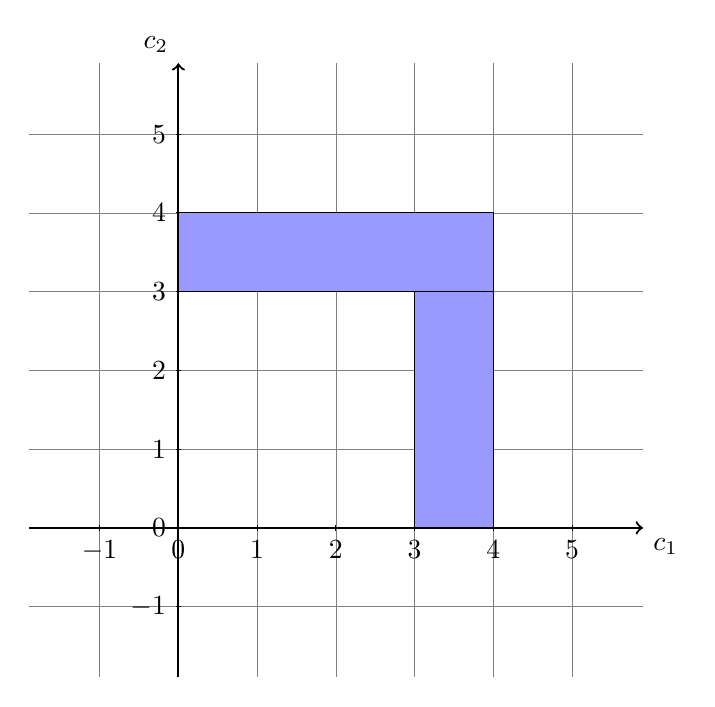
\begin{tikzpicture}
\draw[step=1cm,gray,very thin] (-1.9,-1.9) grid (5.9,5.9);

%\shadedraw[inner color=blue,outer color=red, draw=black] (0,0) rectangle (4,4);

\draw[thick,->] (-1.9,0) -- (5.9,0) node[anchor=north west] {$c_1$};
\draw[thick,->] (0,-1.9) -- (0,5.9) node[anchor=south east] {$c_2$};

\foreach \x in {-1,0,1,2,3,4,5}
    \draw (\x cm,1pt) -- (\x cm,-1pt) node[anchor=north] {$\x$};
\foreach \y in {-1,0,1,2,3,4,5}
    \draw (1pt,\y cm) -- (-1pt,\y cm) node[anchor=east] {$\y$};
    
\filldraw[fill=blue!40!white, draw=black] (0,3) rectangle (4,4);
\filldraw[fill=blue!40!white, draw=black] (3,0) rectangle (4,3);

\end{tikzpicture}
\end{adjustbox}
\caption{After Minus}
\label{fig:after_minus_zone}
\end{subfigure}

\caption{Minus fragmentation}
\label{fig:fragmentation}
\end{figure}